\documentclass[12pt]{article}
\usepackage{graphicx}
\usepackage{float}
  
%
% Title[Enter title of the experiment here]
\title{EE230: Experiment No.7\\
Special Opamp Linear Circuits - Active Filters}

% Author[Enter details of author here]
\author{Aksh Garg, 20D070008}

% begin the document.
\begin{document}

% make a title page.[this creates title page]
\maketitle
 

\section{Overview of the experiment} %[This segment creates Section as seen in document]

\subsection{Aim of the experiment}%[This segment creates sebsections under the same section]

The aim of this experiment is to understand what are different types of active filters, and how we can implement them using opamps and different types of resistors and capacitors. For these filters, we have to find out some parameters, like Bandwidth, CutOff Frequency, or maximum Gain Frequency. To calculate these parameters, there are different different circuits, which we analyse and found out the parameters by getting the output experimentally and doing some calculations. These circuits and calculations are shown in the Design section. These experimental results needs to be compared with the theoritical results.

\subsection{Methods}
First of all, as the circuit diagrams are given to us in the lab document, we make the circuit on the breadboard carefully. After checking the connections, we provide the required power supply to the board wherever required. The output which is required to do the calculations, are measured using Digital Multi-Meter, and the readings are taken. Using these readings, we calculate the required parameter values by doing the required calculations.\\
After that, these experimental values are compared with the theoritical values to check whether our experimental values are approximately same to theoritical values.

\section{Design}%[To add multiple sections, keep appending blocks like this]

\subsection{ Sallen-Key (2-pole) active low-pass filter}
\begin{figure}[H]
\begin{center}
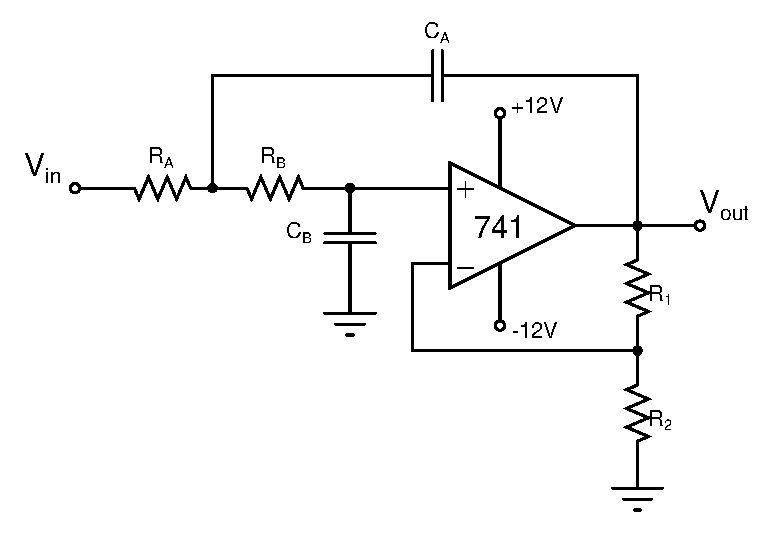
\includegraphics[scale = 0.8]{p1.eps}
\caption{ Sallen-Key (2-pole) active low-pass filter}
\end{center}
\end{figure}
Circuit values: $R_A$ = $R_B$ = 4.7k$\Omega $, $C_A$ = $C_B$ = 0.1uF, $R_1$ = 1.8k$\Omega $, $R_2$ = 3.3k$\Omega $. \\
The above diagram shows the active low-pass filter. This has a higher gain when the input is of low frequency. As we increase the frequency, we reach to a CutOff Frequency, where the $V_{OUT}$ becomes 1/$\sqrt(2) $ times its maximum value. After that, the gain plot has a much sharper roll-off of -40 dB/decade beyond the cut-off frequency. $R_1$ and $R_2$ values are chosen such that $R_1$ = 0.586$R_2$. The calculation for CutOff Frequency is as follows:
\begin{equation}
   f_c = 1/(2\pi RC)
 \end{equation}
R = $R_A$ = $R_B$, C =  $C_A$ =  $C_B$.\\
\textbf{Theoritical Result:} \\
\begin{equation}
    f_c = 1/(2\pi 4.7 10^{-4})
 \end{equation}
\begin{equation}
    f_c = 340Hz
 \end{equation}
So, for this low-pass filter, the above equation will give us thetheoritical value of $f_c$.


\subsection{ Sallen-Key (2-pole) active high-pass filter}
\begin{figure}[H]
\begin{center}
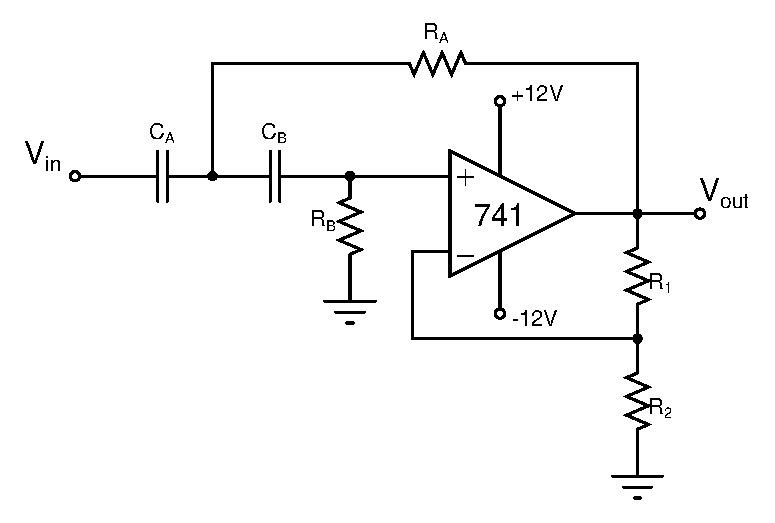
\includegraphics[scale = 0.8]{p2.eps}
\caption{ Sallen-Key (2-pole) active high-pass filter}
\end{center}
\end{figure}
Circuit values: $R_A$ = $R_B$ = 4.7k$\Omega $, $C_A$ = $C_B$ = 0.1uF, $R_1$ = 1.8k$\Omega $, $R_2$ = 3.3k$\Omega $.\\
The above diagram shows the active high-pass filter. This has a lower gain when the input is of low frequency. As we increase the frequency, we reach to a CutOff Frequency, where the $V_{OUT}$ becomes 1/$\sqrt{2} $ times its maximum value. After that, the gain plot has a much sharper roll-off of 40 dB/decade beyond the cut-off frequency. $R_1$ and $R_2$ values are chosen such that $R_1$ = 0.586$R_2$. The calculation for CutOff Frequency is as follows:
\begin{equation}
   f_c = 1/(2\pi RC)
 \end{equation}
R = $R_A$ = $R_B$, C =  $C_A$ =  $C_B$.\\
\textbf{Theoritical Result:} \\
\begin{equation}
    f_c = 1/(2\pi 4.7 10^{-4})
 \end{equation}
\begin{equation}
    f_c = 340Hz
 \end{equation}
So, for this high-pass filter, the above equation will give us thetheoritical value of $f_c$.

\subsection{Multiple-feedback Active Band-Pass Filter}
\begin{figure}[H]
\begin{center}
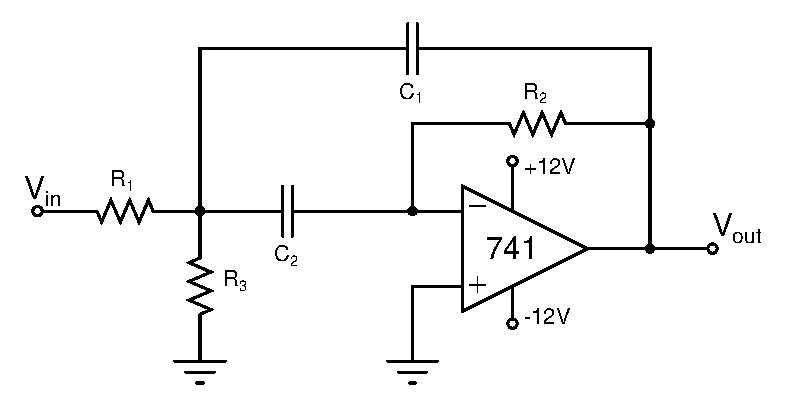
\includegraphics[scale = 0.8]{p3.eps}
\caption{Multiple-feedback Active Band-Pass Filter}
\end{center}
\end{figure}
Circuit values: $R_3$ = 2.7k$\Omega $, $C_1$ = $C_2$ = 0.01uF, $R_1$ = 68k$\Omega $, $R_2$ = 180k$\Omega $.\\
The above diagram shows the Multiple-feedback Active Band-Pass Filter. This has a lower gain when the input is of low frequency. As we increase the frequency, the gain increases. After some frequency, gains reaches to maximum value, after that if we increase the frequency, then gain starts to decrease again. The following equations are used to find the theoritical values:
\begin{equation}
   Q = \pi f_oCR_2
 \end{equation}
\begin{equation}
   BW = f_o/Q
 \end{equation}
\begin{equation}
   f_o = (1/(2\pi C)) * \sqrt{(R_1 + R_2)/(R_1R_2R_3)}
 \end{equation}
\textbf{Theoritical Result:} \\
\begin{equation}
    f_o = 15.92*10*8.66 = 729Hz
 \end{equation}
\begin{equation}
   BW = 1/(\pi CR_2) = 176Hz
 \end{equation}
So,  for this filter, the above equation will give us thetheoritical value of $f_o$ and BW.



\section{Experimental results}

\subsection{ Sallen-Key (2-pole) active low-pass filter}
\begin{table}[H]
		% Center the table
		\begin{center}
		
		\begin{tabular}{|c|c|}
			% To create a horizontal line, type \hline
			\hline
			% To end a column type &
			% For a linebreak type \\
			\textbf{f(in Hz)} & \textbf{$V_{OUT}$ (in V)}\\
			\hline
			10 & 2.56\\
			\hline
			20 & 3.04\\
			\hline
                   30 & 3.12\\
			\hline
                   50 & 3.2\\
			\hline
                   100 & 3.2\\
			\hline
                   200 & 3.2\\
			\hline
300 & 3.2\\
			\hline
400 & 2.72\\
			\hline
450 & 2.48\\
			\hline
470 & 2.24\\
			\hline
500 & 2.16\\
			\hline
600 & 1.76\\
			\hline
700 & 1.28\\
			\hline
800 & 1.12\\
			\hline
            
		\end{tabular}
		\end{center}
\end{table}

Following is the Bode-Plot of the Output:
\begin{figure}[H]
\begin{center}
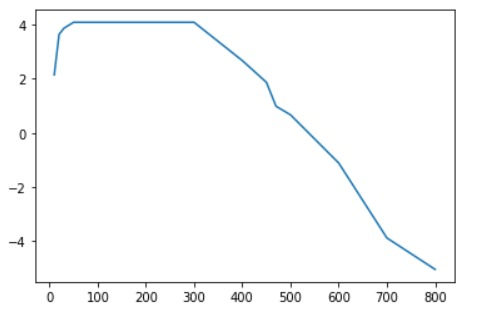
\includegraphics[scale = 0.8]{lowe.jpeg}
\end{center}
\end{figure}


From here, we can see that our experimental $f_c$ is at 470Hz (at which $V_{OUT}$ becomes 3.2/ $\sqrt{2} $).\\
Theoritical $f_c$ is at 338Hz.


\subsection{ Sallen-Key (2-pole) active high-pass filter}
\begin{table}[H]
		% Center the table
		\begin{center}
		
		\begin{tabular}{|c|c|}
			% To create a horizontal line, type \hline
			\hline
			% To end a column type &
			% For a linebreak type \\
			\textbf{f(in Hz)} & \textbf{$V_{OUT}$ (in V)}\\
			\hline
			10 & 0.16\\
			\hline
			50 & 0.16\\
			\hline
                   100 & 0.32\\
			\hline
                   150 & 0.48\\
			\hline
200 & 0.64\\
			\hline
250 & 0.96\\
			\hline
300 & 1.28\\
			\hline
350 & 1.6\\
			\hline
400 & 1.92\\
			\hline
450 & 2.08\\
			\hline
480 & 2.24\\
			\hline
500 & 2.24\\
			\hline
600 & 2.56\\
			\hline
750 & 2.8\\
			\hline
1000 & 2.96\\
			\hline
1500 & 3.12\\
			\hline
2000 & 3.12\\
			\hline

            
		\end{tabular}
		\end{center}
\end{table}

Following is the Bode-Plot of the Output:
\begin{figure}[H]
\begin{center}
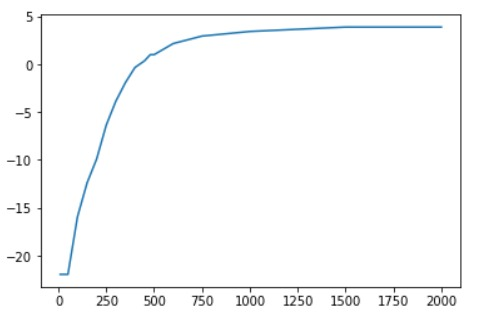
\includegraphics[scale = 0.8]{highe.jpeg}
\end{center}
\end{figure}

From here, we can see that our experimental $f_c$ is at 480Hz (at which $V_{OUT}$ becomes 3.12/ $\sqrt{2} $).\\
Theoritical $f_c$ is at 338Hz.

\subsection{Multiple-feedback Active Band-Pass Filter}
\begin{table}[H]
		% Center the table
		\begin{center}
		
		\begin{tabular}{|c|c|}
			% To create a horizontal line, type \hline
			\hline
			% To end a column type &
			% For a linebreak type \\
			\textbf{f(in Hz)} & \textbf{$V_{OUT}$ (in V)}\\
			\hline
			10 & 0.16\\
			\hline
			50 & 0.16\\
			\hline
                   100 & 0.16\\
			\hline
                   110 & 0.24\\
			\hline
                   150 & 0.32\\
			\hline
200 & 0.32\\
			\hline
300 & 0.48\\
			\hline
350 & 0.64\\
			\hline
400 & 0.8\\
			\hline
450 & 1.04\\
			\hline
500 & 1.36\\
			\hline
530 & 1.76\\
			\hline
550 & 1.92\\
			\hline
600 & 2.24\\
			\hline
650 & 2.24\\
			\hline
670 & 2.24\\
			\hline
700 & 1.92\\
			\hline
724 & 1.76\\
			\hline
750 & 1.6\\
			\hline
800 & 1.28\\
			\hline
900 & 0.96\\
			\hline
1000 & 0.8\\
			\hline
1100 & 0.64\\
			\hline
1250 & 0.64\\
			\hline
1300 & 0.56\\
			\hline
1350 & 0.48\\
			\hline
1500 & 0.48\\
			\hline

		\end{tabular}
		\end{center}
\end{table}

Following is the Bode-Plot of the Output:
\begin{figure}[H]
\begin{center}
\includegraphics[scale = 0.8]{passe.jpeg}
\end{center}
\end{figure}

From here, we can see that our experimental $f_o$ is at 670Hz (at which $V_{OUT}$ becomes 2.24V). \\
BW = 724Hz - 530Hz\\
So, our BandWidth is 194Hz.\\
Theoritical $f_o$ is at 729Hz.\\
Theoritical BW is 176Hz.\\


\section{Experiment completion status}
All the parts of this experiment are completed successfully.

  

\end{document}
